\documentclass[12pt]{article}
\usepackage{mathptmx}
\usepackage{graphicx}

\renewcommand{\baselinestretch}{1.5}
\begin{document}


\section{Abstract} \label{sec:abstract}
The aim of this project is to create a proof-of-concept model for an autonomous robot using artificial intelligence. Reinforcement learning methods will be implemented by making use of models incorporating artificial neural networks.

Conventionally, obstacle avoidance has been implemented using a procedural approach that makes use of predefined values; that are arrived at by means of trial and error, largely. To eliminate the need for inaccurate and hard-to-determine fixed threshold values, we use Artificial Intelligence (hereinafter referred to solely as AI).

All processing shall be done using an on-board computer, in this case a Raspberry Pi 3 Model B. An ultrasonic sensor will be mounted on a servo to read distances. A camera will be mounted to recognize and react to visual stimuli in the form of STOP or GO signs and signals. Using Digital Image Processing (also performed on the Pi), these can be recognized and reacted to. 

Initially there will be zero knowledge present, and unsupervised learning will be performed. The robot will be set to default to forward movement until it collides with an obstacle while maintaining a buffer of all sensor readings at all time and then reads from the buffer every time a collision is made to learn the conditions at which collisions occur.

Collision detection will be done using accelerometer values of the Inertial Measurement Unit (IMU). A mood variable will be used to keep track of collision by attaching a negative weight for every collision and positive increments for uninterrupted forward propagation as an implementation of semi-supervised learning. The cause and effect relation between collision and mood will then be the foundation for collision avoidance. Optimal path can be extrapolated by calculating the local maximum of the longest bitonic sub sequence in the array of distance readings taken in a sweep of the servo with the ultrasonic sensor mounted on top.

Once obstacle avoidance is trained we can incorporate image and speech processing for inputs. Speed breakers can be crossed with adaptive speed. Variable PWM can be given for climbing slopes at a constant speed. Lights can be turned on automatically in the dark. 
However self preservation in the vein of Isaac Asimov's laws of robotics can be implemented by letting the robot disobey a user command that puts the robot in the way of harm. 

By the end of this project we aim to have an elementary exhibit of a truly autonomous self-driving car capable of making realtime decisions without human intervention.

\newpage

\section{List of Tables and Figures} \label{sec:tabfig}

\vfill

\begin{table} [!h]
	\centering
List of tables \\
\vspace{5mm}
		\begin{tabular} {|c|c|c|} \hline
Sr. No. & Particulars & Page No. \\ \hline
1 & Blah & 2 \\
2 & blah & 3 \\ \hline
		\end{tabular}
			\label{tab:ListOfTables}
\end{table}

\vfill

\begin{table} [!h]
	\centering
List of figures \\
\vspace{5mm}
		\begin{tabular} {|c|c|c|} \hline
Sr. No. & Particulars & Page No. \\ \hline
1 & Blah & 2 \\
2 & blah & 3 \\ \hline
		\end{tabular}
			\label{tab:ListOfFigures}
\end{table}

\vfill


\newpage

\section{Introduction} \label{sec:introduction}

The Autonomous Learning Robot provides an excellent opportunity to demonstrate the techniques and methods of Artificial Intelligence. It efficiently utilizes the application of various AI themes like Vision, Learning and autonomous Agent based task accomplishment. Artificial Intelligence is an upcoming field that has attracted research attention and under active development. Owing to this development the resources required to learn and implement its concepts, on an individual user’s scale, have now become accessible. In the process of learning we aim to build upon existing systems, taking a step towards Artificial General Intelligence.

The project will employ concepts from Dynamic Programming for path calculation, Artificial Neural Networks for Machine Learning as a part of Artificial Intelligence, Computer Vision using Digital Image Processing, Natural Language Processing for Speech Recognition, Spatial Mapping to analyze environmental risk of execution of user commands.

Open AI is a non-profit artificial intelligence (AI) research company, associated with business magnate Elon Musk, that aims to carefully promote and develop open-source friendly AI in such a way as to benefit, rather than harm, humanity as a whole. The organization aims to "freely collaborate" with other institutions and researchers by making its patents and research open to the public.

Repurposing industrial robots for daily tasks using machine learning is one branch of OpenAI’s current work. At national level also, research is conducted by Artificial Intelligence Association of India (AIAI) on theory, design, application, and development of the mechanisms underlying thought and intelligent behavior and their embodiment in machines emphasizing intelligent agent systems, knowledge engineering, language technologies, cognitive systems, robotics and human-computer interaction in which these paradigms are contained.

Currently, most hardware oriented applications consist of a procedural approach towards implementation of autonomy. However, Artificial Narrow Intelligence is being integrated at a rapid rate. We aim to initiate a transition towards Artificial General Intelligence by expanding upon the avenues to which ANI is being applied and coalescing these into a step in the direction of AGI. 





\newpage

\section{Need of Project} \label{sec:need}

A robot is a container for AI, sometimes mimicking the human form, sometimes not�but the AI itself is the computer inside the robot. AI is the brain, and the robot is its body�if it even has a body. For example, the software and data behind Siri is AI, the woman�s voice we hear is a personification of that AI, and there�s no robot involved at all.

The term "`Singularity"'  has been used in math to describe an asymptote-like situation where normal rules no longer apply. It�s been used in physics to describe a phenomenon like an infinitely small, dense black hole or the point we were all squished into right before the Big Bang. Again, situations where the usual rules don�t apply. 

There are many different types or forms of AI since AI is a broad concept, the critical categories we need to think about are based on an AI�s caliber. There are three major AI caliber categories:

\begin{itemize}
	\item Artificial Narrow Intelligence (ANI): Sometimes referred to as Weak AI, Artificial Narrow Intelligence is AI that specializes in one area. There�s AI that can beat the world chess champion in chess, but that�s the only thing it does. Ask it to figure out a better way to store data on a hard drive, and it�ll look at you blankly.
	\item Artificial General Intelligence (AGI): Sometimes referred to as Strong AI, or Human-Level AI, Artificial General Intelligence refers to a computer that is as smart as a human across the board�a machine that can perform any intellectual task that a human being can. Creating AGI is a much harder task than creating ANI, and we�re yet to do it. Professor Linda Gottfredson describes intelligence as �a very general mental capability that, among other things, involves the ability to reason, plan, solve problems, think abstractly, comprehend complex ideas, learn quickly, and learn from experience.� AGI would be able to do all of those things as easily as you can.
	\item Artificial Superintelligence (ASI): Oxford philosopher and leading AI thinker Nick Bostrom defines superintelligence as �an intellect that is much smarter than the best human brains in practically every field, including scientific creativity, general wisdom and social skills.� Artificial Superintelligence ranges from a computer that�s just a little smarter than a human to one that�s trillions of times smarter�across the board. ASI is the reason the topic of AI is such a spicy meatball and why the words �immortality� and �extinction� will both appear in these posts multiple times.
\end{itemize}

As of now, humans have conquered the lowest caliber of AI-ANI-in many ways, and it�s everywhere. The AI Revolution is the road from ANI, through AGI, to ASI�a road we may or may not survive but that, either way, will change everything.
\vspace{5mm}
Nothing will make you appreciate human intelligence like learning about how unbelievably challenging it is to try to create a computer as smart as we are. Building skyscrapers, putting humans in space, figuring out the details of how the Big Bang went down�all far easier than understanding our own brain or how to make something as cool as it. As of now, the human brain is the most complex object in the known universe. What�s interesting is that the hard parts of trying to build AGI are not intuitively what you�d think they are. 

What you quickly realize when you think about this is that those things that seem easy to us are actually unbelievably complicated, and they only seem easy because those skills have been optimized in us (and most animals) by hundreds of millions of years of animal evolution. When you reach your hand up toward an object, the muscles, tendons, and bones in your shoulder, elbow, and wrist instantly perform a long series of physics operations, in conjunction with your eyes, to allow you to move your hand in a straight line through three dimensions. It seems effortless to you because you have perfected software in your brain for doing it. Same idea goes for why it�s not that malware is dumb for not being able to figure out the slanty word recognition test when you sign up for a new account on a site�it�s that your brain is super impressive for being able to.

On the other hand, multiplying big numbers or playing chess are new activities for biological creatures and we haven�t had any time to evolve a proficiency at them, so a computer doesn�t need to work too hard to beat us.

The idea of AGI is that we�d build a computer whose two major skills would be doing research on AI and coding changes into itself�allowing it to not only learn but to improve its own architecture. We�d teach computers to be computer scientists so they could bootstrap their own development. And that would be their main job�figuring out how to make themselves smarter.

\newpage

\section{Literature Survey} \label{sec:litsurvey}

Supervised Learning: \\

In supervised learning, we are given a data set and already know what our correct output should look like, having the idea that there is a relationship between the input and the output.

Supervised learning problems are categorized into "regression" and "classification" problems. In a regression problem, we are trying to predict results within a continuous output, meaning that we are trying to map input variables to some continuous function. In a classification problem, we are instead trying to predict results in a discrete output. In other words, we are trying to map input variables into discrete categories.

Example:

Given data about the size of houses on the real estate market, try to predict their price. Price as a function of size is a continuous output, so this is a regression problem.

We could turn this example into a classification problem by instead making our output about whether the house "sells for more or less than the asking price." Here we are classifying the houses based on price into two discrete categories. \\

\vspace{5mm}
Unsupervised Learning: \\

Unsupervised learning allows us to approach problems with little or no idea what our results should look like. We can derive structure from data where we don't necessarily know the effect of the variables.

We can derive this structure by clustering the data based on relationships among the variables in the data.

With unsupervised learning there is no feedback based on the prediction results.

Example:

Clustering: Take a collection of 1,000,000 different genes, and find a way to automatically group these genes into groups that are somehow similar or related by different variables, such as lifespan, location, roles, and so on.

Non-clustering: The "Cocktail Party Algorithm", allows you to find structure in a chaotic environment. (i.e. identifying individual voices and music from a mesh of sounds at a cocktail party).

\vspace{5mm}



\newpage

\section{Objectives} \label{sec:objectives}

\begin{itemize}
  \item To create a proof-of-concept model for a learning robot using Artificial Intelligence performing obstacle avoidance with better accuracy than the conventional system. 
	\vspace{5mm}
	\item To eliminate the need for inaccurate and hard-to-determine fixed threshold values.
	\vspace{5mm}
	\item A system that will be able to integrate a learning based module to adapt to any hardware environment.
\vspace {5mm} 
\item To incorporate image and speech processing modules for input.
		
\end{itemize}

\newpage

\section{Methodology} \label{sec:methodology}



\newpage

\section{Flow Charts} \label{sec:flowcharts}

\vfill
\begin{figure} [!h]
	\centering
	\caption{Crash Based Learning Module}
		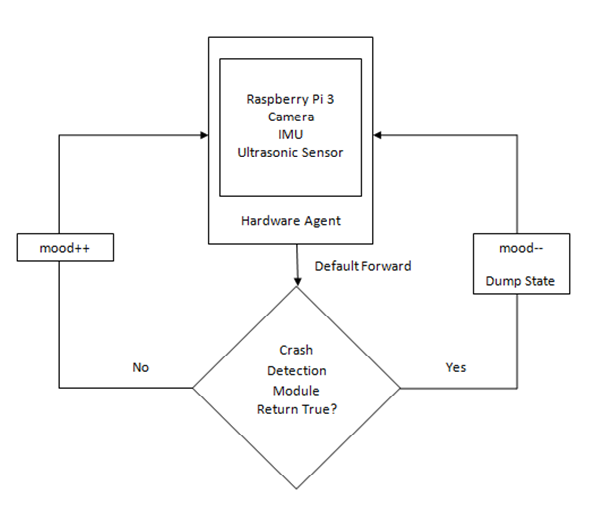
\includegraphics{flow_1.png}
	\label{fig:flow 1}
\end{figure}
\vfill

\newpage

\vfill
\begin{figure} [!h]
	\centering
	\caption{Optimal path Calculate and Collision Avoidance Module}
		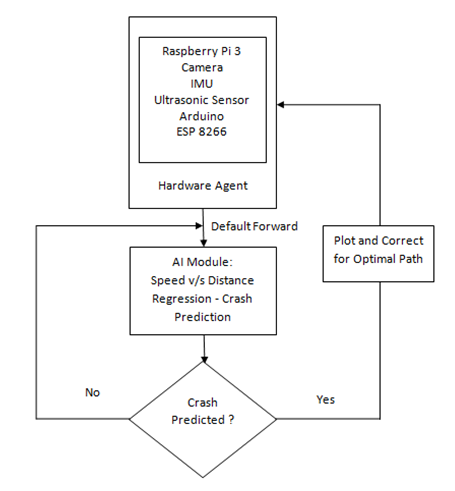
\includegraphics{flow_2.png}
	\label{fig:flow 2}
\end{figure}
\vfill

\newpage

\section{Data Flow Diagrams} \label{sec:dfd}

\vfill

\begin{figure} [!h]
	\centering
	\caption{Level 0 DFD}
		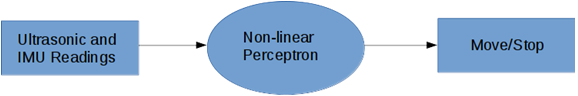
\includegraphics{dfd_1.png}
	\label{fig:dfd 1}
\end{figure}
\vfill

\begin{figure} [!h]
	\centering
	\caption{Level 1 DFD}
		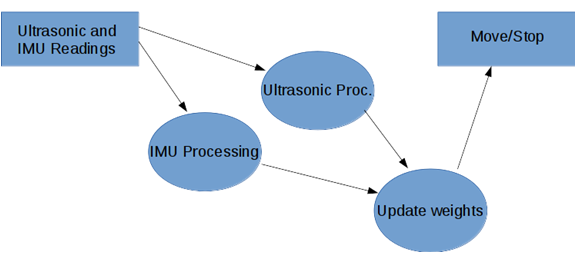
\includegraphics{dfd_2.png}
	\label{fig:dfd 2}
\end{figure}

\vfill

\end{document}